\subsubsection{BOUT opsætning}
BOUT++ og BOUT-HESEL blev opsat på DTU's HPC-cluster i et separat softwaremiljø, hvor de nødvendige moduler for MPI, FFTW, NetCDF og Intel compiler først blev loadet. Dette var nødvendigt, fordi både kompilering og kørsel af simuleringerne afhænger af parallelisering og eksterne numeriske biblioteker. Derudover blev \texttt{OMP\_NUM\_THREADS} sat til 16, så opsætningen matchede den ønskede brug af clusterets CPU-ressourcer.

Selve installationen blev udført i to trin. Først blev BOUT++ klonet fra det officielle repository, sat til version \texttt{v4.3.2}, konfigureret med \texttt{./configure} og derefter kompileret med \texttt{make -j16}. BOUT++ fungerer her som den generelle simuleringsramme, som håndterer numerisk løsning, gitterstruktur og parallel udførelse. Herefter blev BOUT-HESEL klonet med tilhørende submoduler. I denne del af opsætningen blev de nødvendige komponenter fra \texttt{HESEL-Common} koblet til projektet, så HESEL-modellen kunne bygges oven på den allerede kompilerede BOUT++-installation. Til sidst blev BOUT-HESEL også kompileret med \texttt{make -j16}.

Når både BOUT++ og BOUT-HESEL var bygget, kunne simuleringerne køres med \texttt{mpirun -np 4 ./hesel -d <folder med BOUT.inp fil>}. Her læser programmet sin konfiguration fra den tilhørende \texttt{BOUT.inp}-fil, som specificerer blandt andet gitteropløsning, tidsstep, randbetingelser og fysiske parametre. Denne opsætning gjorde det muligt at generere konsistente HESEL-simuleringer på clusteret, som efterfølgende kunne bruges som datagrundlag for de læringsbaserede modeller.
Dette projekts opsætning af BOUT++ og BOUT-HESEL er dokumenteret i detaljer i filen $\texttt{skriftlig\_arbajde/opsaetning}$, hvor alle nødvendige kommandoer og trin er gennemgået for at sikre reproducerbarhed.


\subsubsection{Data generaring} \label{ch4_1_1}
Til dette er der generet 6 simuleringer. Herfra er 3 standard simuleringer og 3 simuleringer hvor eneste ændring er: tidsteppet, fysikken og grid opløsningen.
Alle simulerings konfigurations filer der bestemmer begyndelsestilstande, randbetingleser,
grid opløsninger, fysiske parametre og tilfældige seed ligger i folderen $\texttt{sim\_data}$ i Github repositoryet.
\begin{itemize}
    \item 3 standard simuleringer starter med $\texttt{sim\_data/Alexander\_*}$ " Her er * en plads for forskellige seed"
    \item Folderen med modificeret tidsteppet hedder $\texttt{sim\_data/Alexander\_\_t\_n}$
    \item Folderen med modificeret fysik hedder $\texttt{sim\_data/Alexander\_\_fys\_R\_1}$
    \item Folderen med modificeret grid opløsning hedder $\texttt{sim\_data/Alexander\_\_grid\_c\_0}$
\end{itemize}

Alle input filer i $\texttt{sim\_data/Alexander\_*/BOUT.inp}$.
Alle simulerninger blev udført på Danmarks Tekniske Universitet (DTU)'s High Performance Computing (HPC) cluster, med 16 CPU kerner.
Hver simulering tog ikke længere end 1 time.
Submit filen til simuleringen ligger her: $\texttt{sim\_data/submit\_simulering.sh}$.
Træningen af modellerne blev udført lokalt. Derofr blev filer downloadet fra HPC clusteret til lokal maskine med 
\[
    \texttt{rsync -avh --progress ssh:<sti til data> <sti til lokal folder>}
\]
Det er ikke forvæntet at download skule ødelegge data'en når den komprimeres og downloades med rsync.

For simuleringen med modificeret tidstep sættes variablen $\texttt{timestep = 25}$. Det betyder at modellen skal forudsige længere frem
i tiden end hvad den er trænet på.

For simuleringen med modificeret fysik er følgende variabler ændret til
\begin{align*}
    &\texttt{Z\_eff  = 1.7} \\
    &\texttt{Bt      = 2.32} \\
    &\texttt{Te0     = 75.6} \\
    &\texttt{Ti0     = 75.6} \\
\end{align*}
Disse blev vurderet til at være mest almindelige fysiske parametre at variere.
For simuleringen med modificeret grid opløsning blev ændre til at være $\texttt{nx = 514}, \texttt{nz = 512}$

Alle filer, både standard og modificerede, havde forskellige seeds for at sikre at udviklingen af simuleringerne var forksellige. Dette gav følgende længer af simuleringer:
\begin{table}[H]
    \centering
    \begin{tabular}{lrr}
        \toprule
        simulation & $t_{\text{end}}$ & $t_{\text{idx}}$ \\
        \midrule
        \texttt{pi}   & 15015 & 1001 \\
        \texttt{e}    & 14055 & 937  \\
        \texttt{phi\_0}& 11130 & 742  \\
        \texttt{\_t\_n} & 17950 & 718  \\
        \texttt{\_fys\_R\_1} & 7665 & 511  \\
        \texttt{\_grid\_c\_0} & 7155 & 477  \\
        \bottomrule
    \end{tabular}
    \caption{Længden af simuleringerne i Bohm normaliserede tidsenheder og antal tidsindekser.}
    \label{tab:sim_times}
\end{table}
Det bemærkes at alle standard simuleringerne og simuleringen med modificeret tidstep var længere end simuleringerne med modificeret fysik og grid opløsning. Der blev
generet flere filer med modificeret fysik og grid men dette var blot de simuleringer der kom længst.


\subsubsection{Data visualisering}
Selve visualiseringen af data er udført i $\texttt{hesel\_scraper/visualizer.ipynb}$.
Til indlæsning af simuleringsdata anvendes klassen $\texttt{BOUTHESELInfo}$ fra biblioteket $\texttt{bout\_dump}$.
Klassen benytter $\texttt{xbout}$ til at læse de parallelle outputfiler fra hver data folder, hvor simuleringsdomænet er opdelt i flere subdomæner,
ét for hver processor. Disse subdomæner sammensættes automatisk til det oprindelige globale gitter, hvorefter data lagres som PyTorch tensorer.

Det første billede genereret er begyndelsestilstanden for hvert felt, som set i \ref{fig:hesel_profiles}. Hvert felt er udvidet symetrisk om $z$-aksen.
For felterne $n$, $p_e$ og $p_i$ tages logaritmen, og $\omega^*$ er initialiseret til 0 og $\phi$ er udregnet med formelen \eqref{eq: vorticitet funktionen}.
For det første billede genereret tilføjes der også en lille tilfældig støj så alle simuleringer udvikler sig forskelligt over tid. Denne støj er ikke synlig i $t=0$.
Den vertikale bar ved siden af hver felt viser farveskalaen for det pågældende felt.
Dette giver følgende billeder.

\begin{figure}[H]
    \centering
    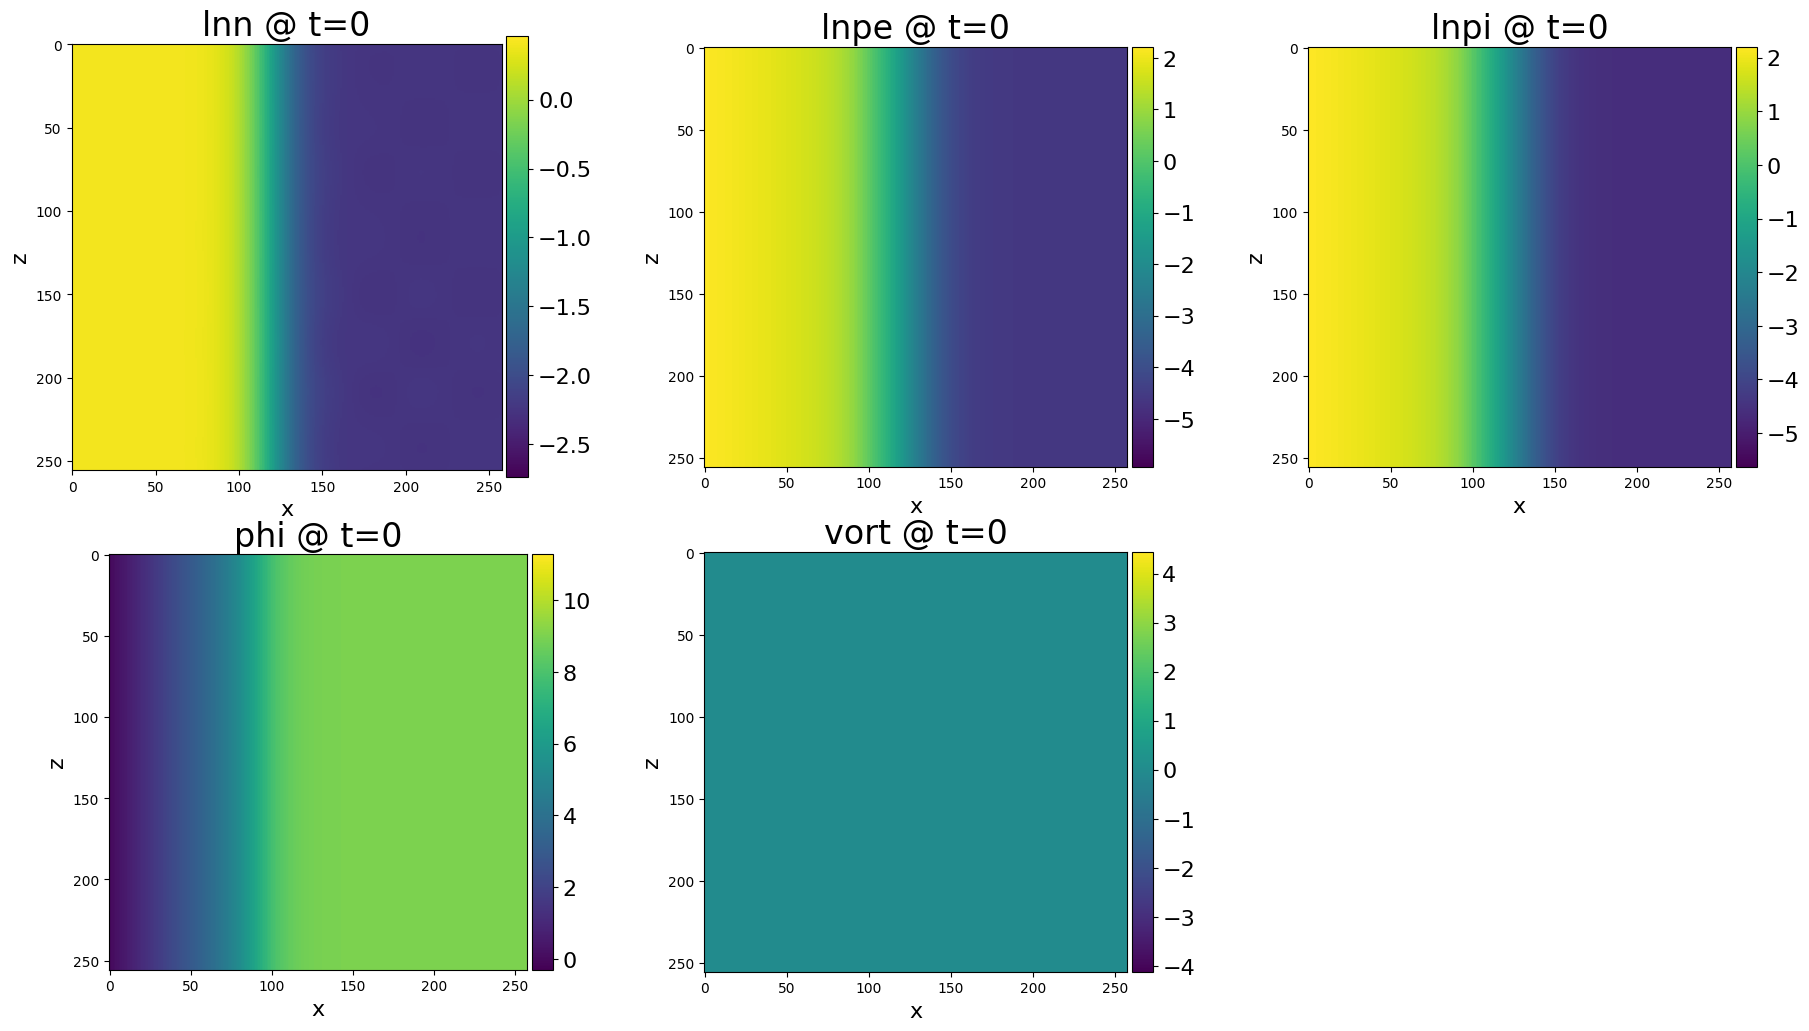
\includegraphics[width=0.8\textwidth]{figures/Standard_fields/_Alexander_pi_samlet_0.png}
    \caption{Standard simuleringen $\texttt{Alexander\_pi}$ til $t=0$. Akserne er i numeriske grid enheder og ghost cells inkluderet.
    Fysiske enheder er $z = 140/\rho_s$, $x = 140/\rho_s + ghostcells$}
    \label{fig: Alexander pi 0}
\end{figure}
\begin{figure}[H]
    \centering
    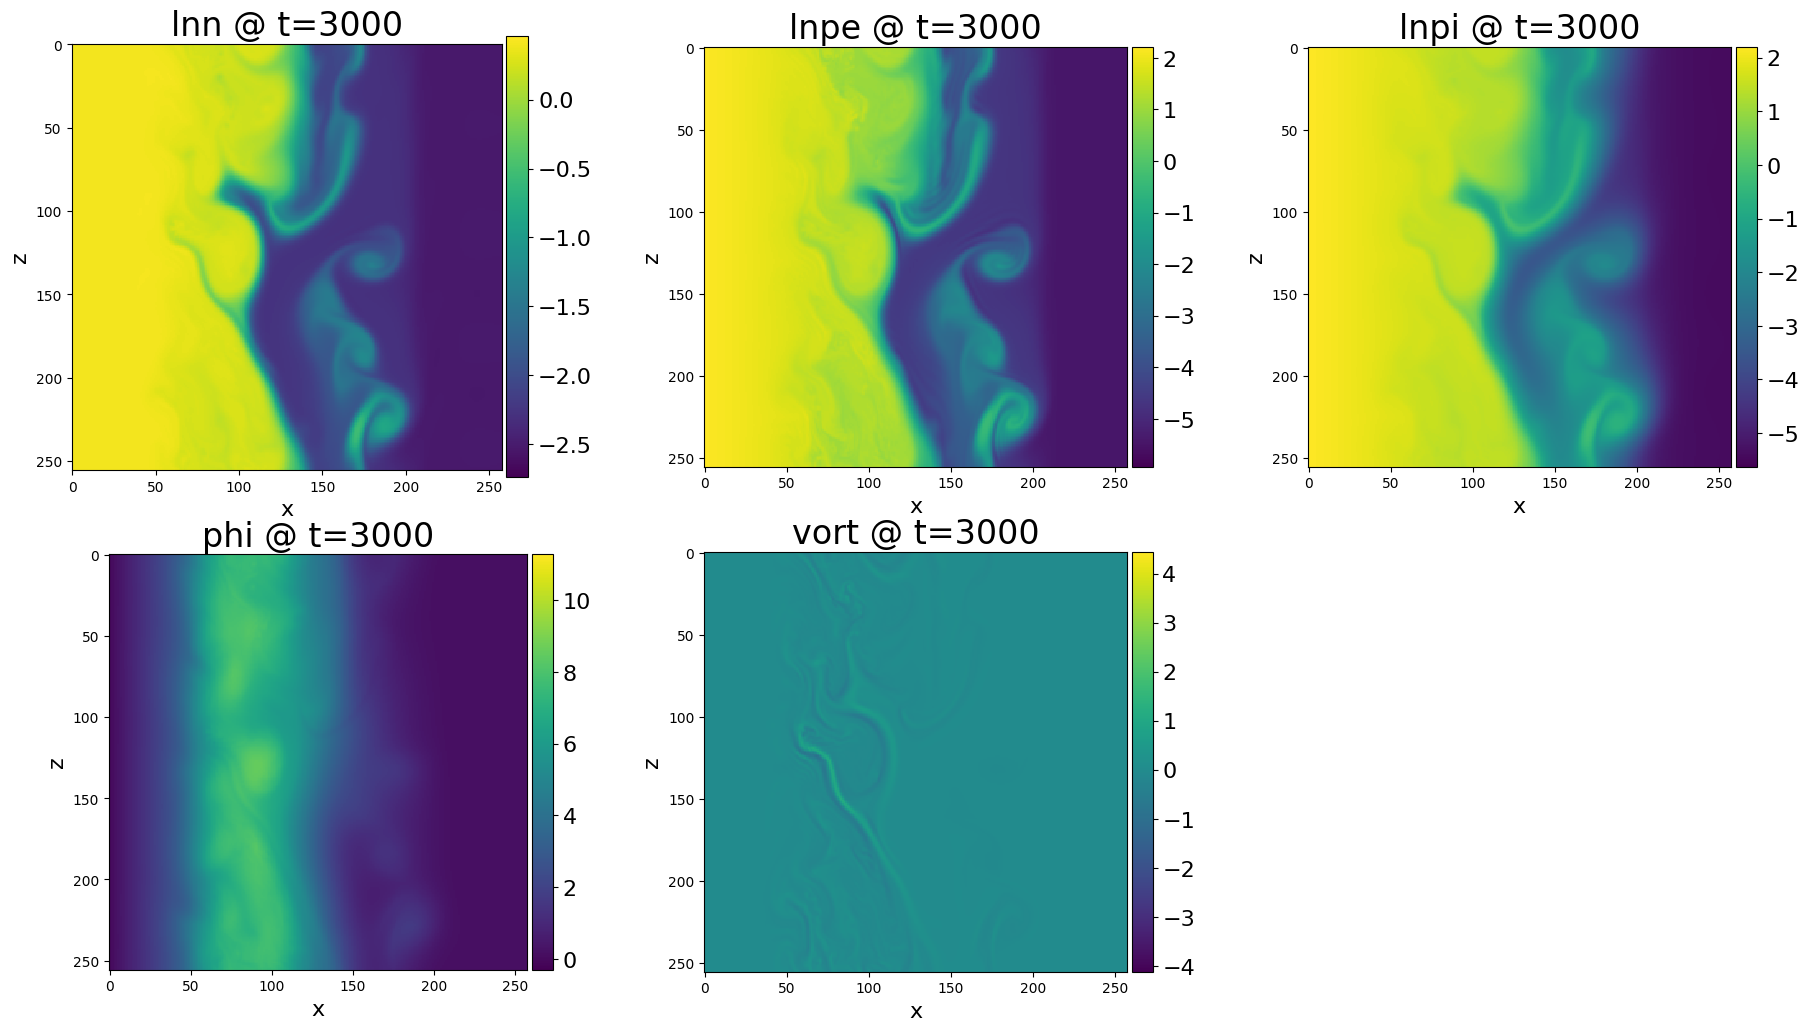
\includegraphics[width=0.8\textwidth]{figures/Standard_fields/_Alexander_pi_samlet_200.png}
    \caption{Standard simuleringen $\texttt{Alexander\_pi}$ til $t=3000$. Akserne er i numeriske grid enheder og ghost cells inkluderet.
    Fysiske enheder er $z = 140/\rho_s$, $x = 140/\rho_s + ghostcells$}
    \label{fig: Alexander pi 3000}
\end{figure}

For tidsudviklingen af feltet ln(n) for udvalgte simuleringer, se \ref{fig: Alexander ln(n) tidsudvikling}. Her blev der udvalgt 2 standard simuleringer og 
simuleringen af modificeret fysik, og modificeret grid opløsning. Da simuleringerne af modificeret tidstep og den sidste standard simulering har samme fysik
og gridopløsning er disse undladt at have med. Ellers kan alle billederne ses i folderen $\texttt{billeder}$. Hvis man har simuleringsdataen kan man 
bruge $\texttt{hesel\_scraper/visualizer.ipynb}$ til se udviklingen af alle felter for én simulering.
